\section{Testing}												
\label{sec:Testing}
\paragraph{} Because we chose an incremental model as a life cycle model so the most testing is done during each increment after its implementation phase. So when everything was implemented, the developer then tested the entire application.
\par The Android application had no formal unit testing, in large part due to the complex nature of image keypointing.  Nonetheless, the system was heavily user tested and demonstrated reasonable performance. During the user testing, several interface issues and functionalities were improved. For example, the titles on each page were not same but were made to be consistent; the system \bsq{back} button was made to exit the application when pressed at the main page; the \bsq{find} button was made to only be activated once; and the \bsq{cancel} button was added when finding a gift.  
\par As mentioned, the image recognition functionalities for the Android application were not easily tested. To make sure the region we found was correct, we took sent numerous gifts using a variety of background images.  We then attempted to find these gifts by scanning from a variety of angles, distances, and phone orientations. An example is shown in Figure \ref{AnExampleForFindingAGift}.
\begin{figure}[htb]
\centering
\begin{minipage}[H]{0.3\textwidth}
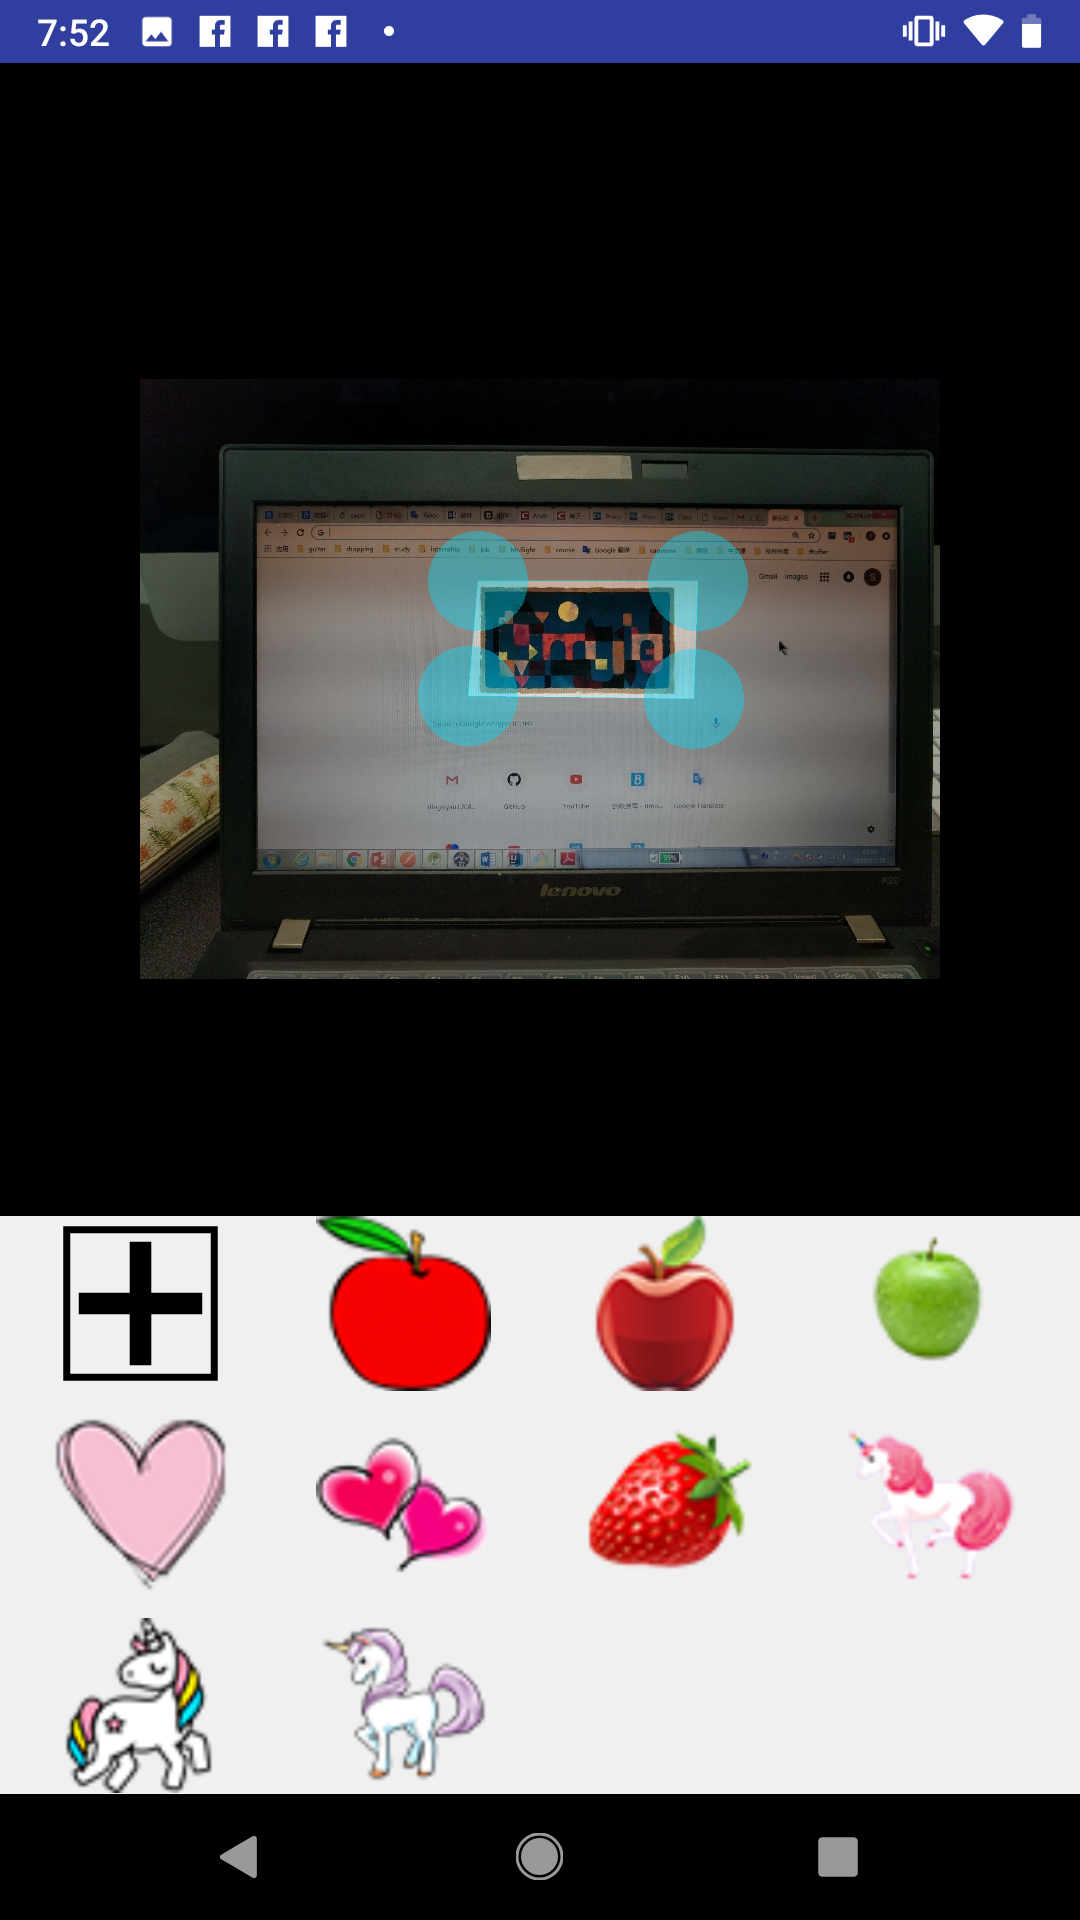
\includegraphics[width=.95\textwidth]{section05/assets/resultExample2.png}
\subcaption{\label{RegionSelected}}
\end{minipage}%
\begin{minipage}[H]{0.3\textwidth}
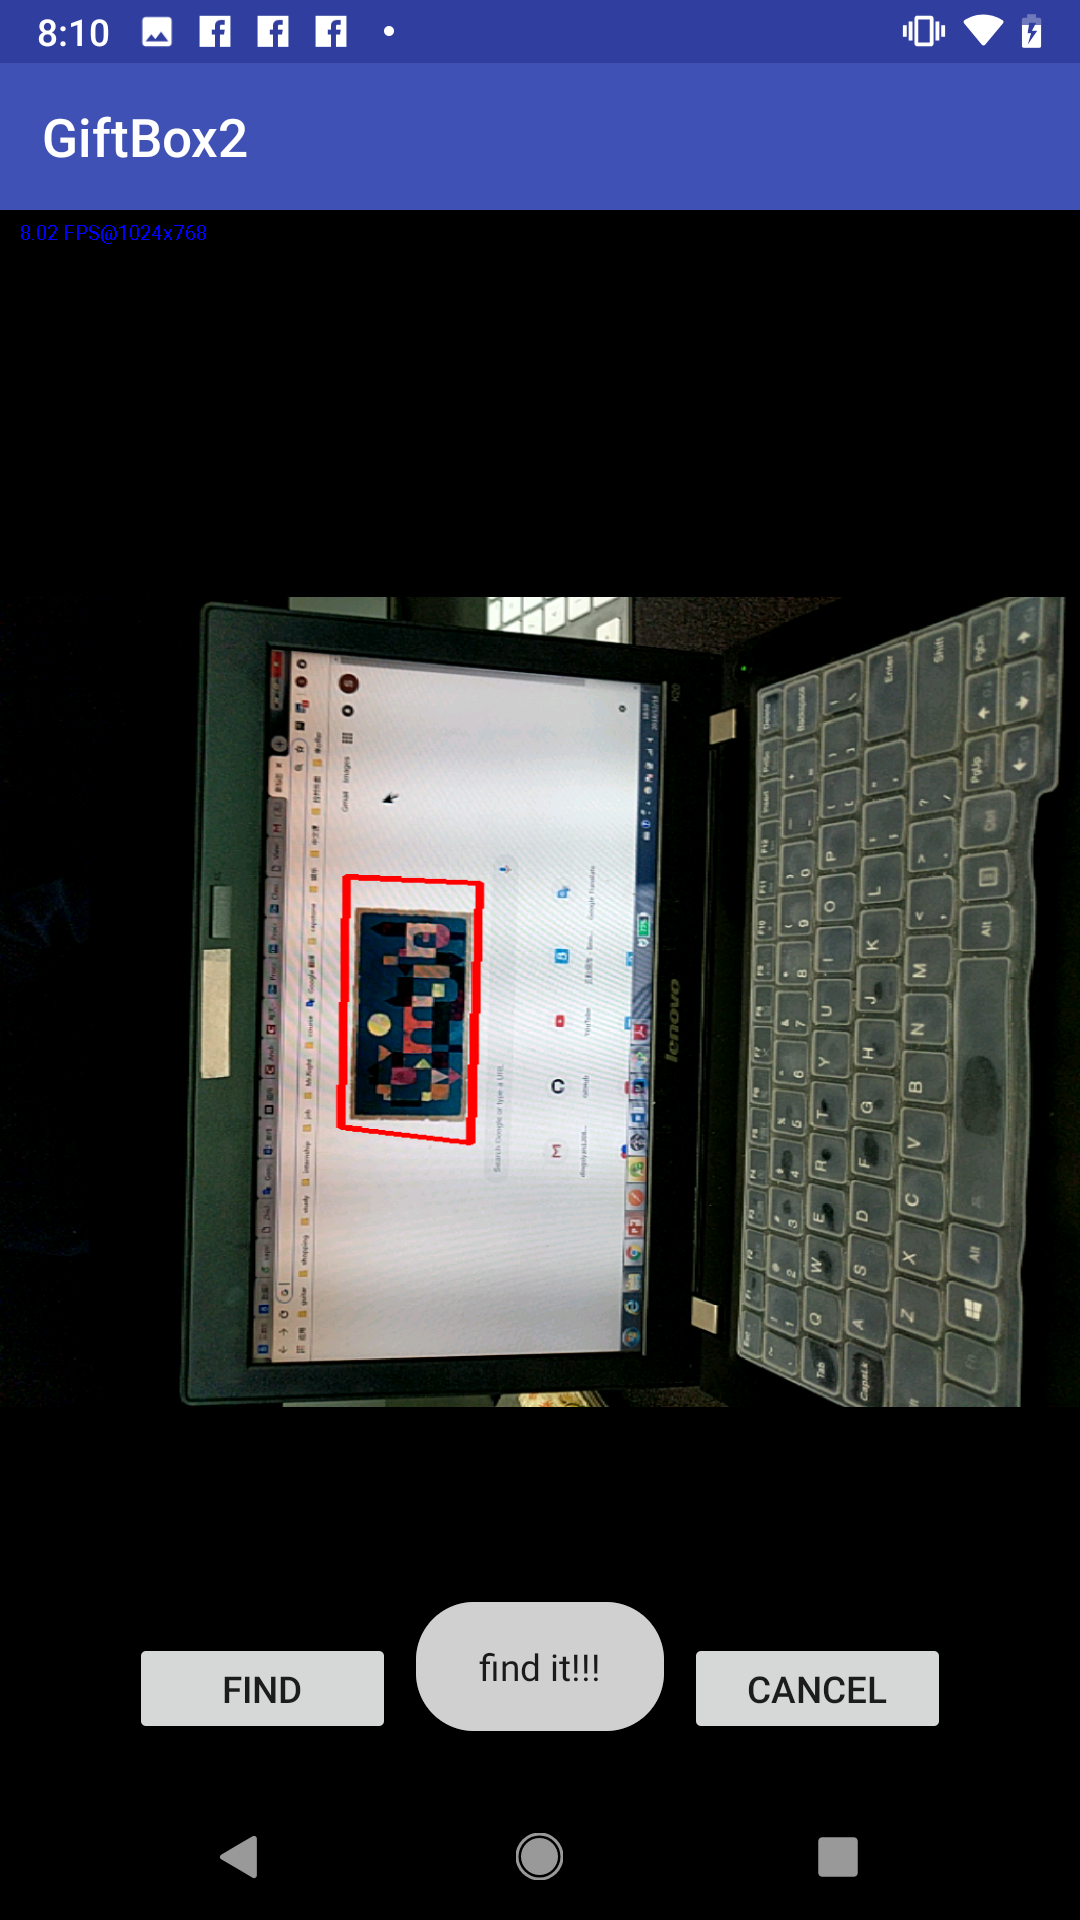
\includegraphics[width=.95\textwidth]{section05/assets/resultExample3.png}
\subcaption{\label{DetectedRegionCorrect1}}
\end{minipage}%

\begin{minipage}[H]{0.3\textwidth}
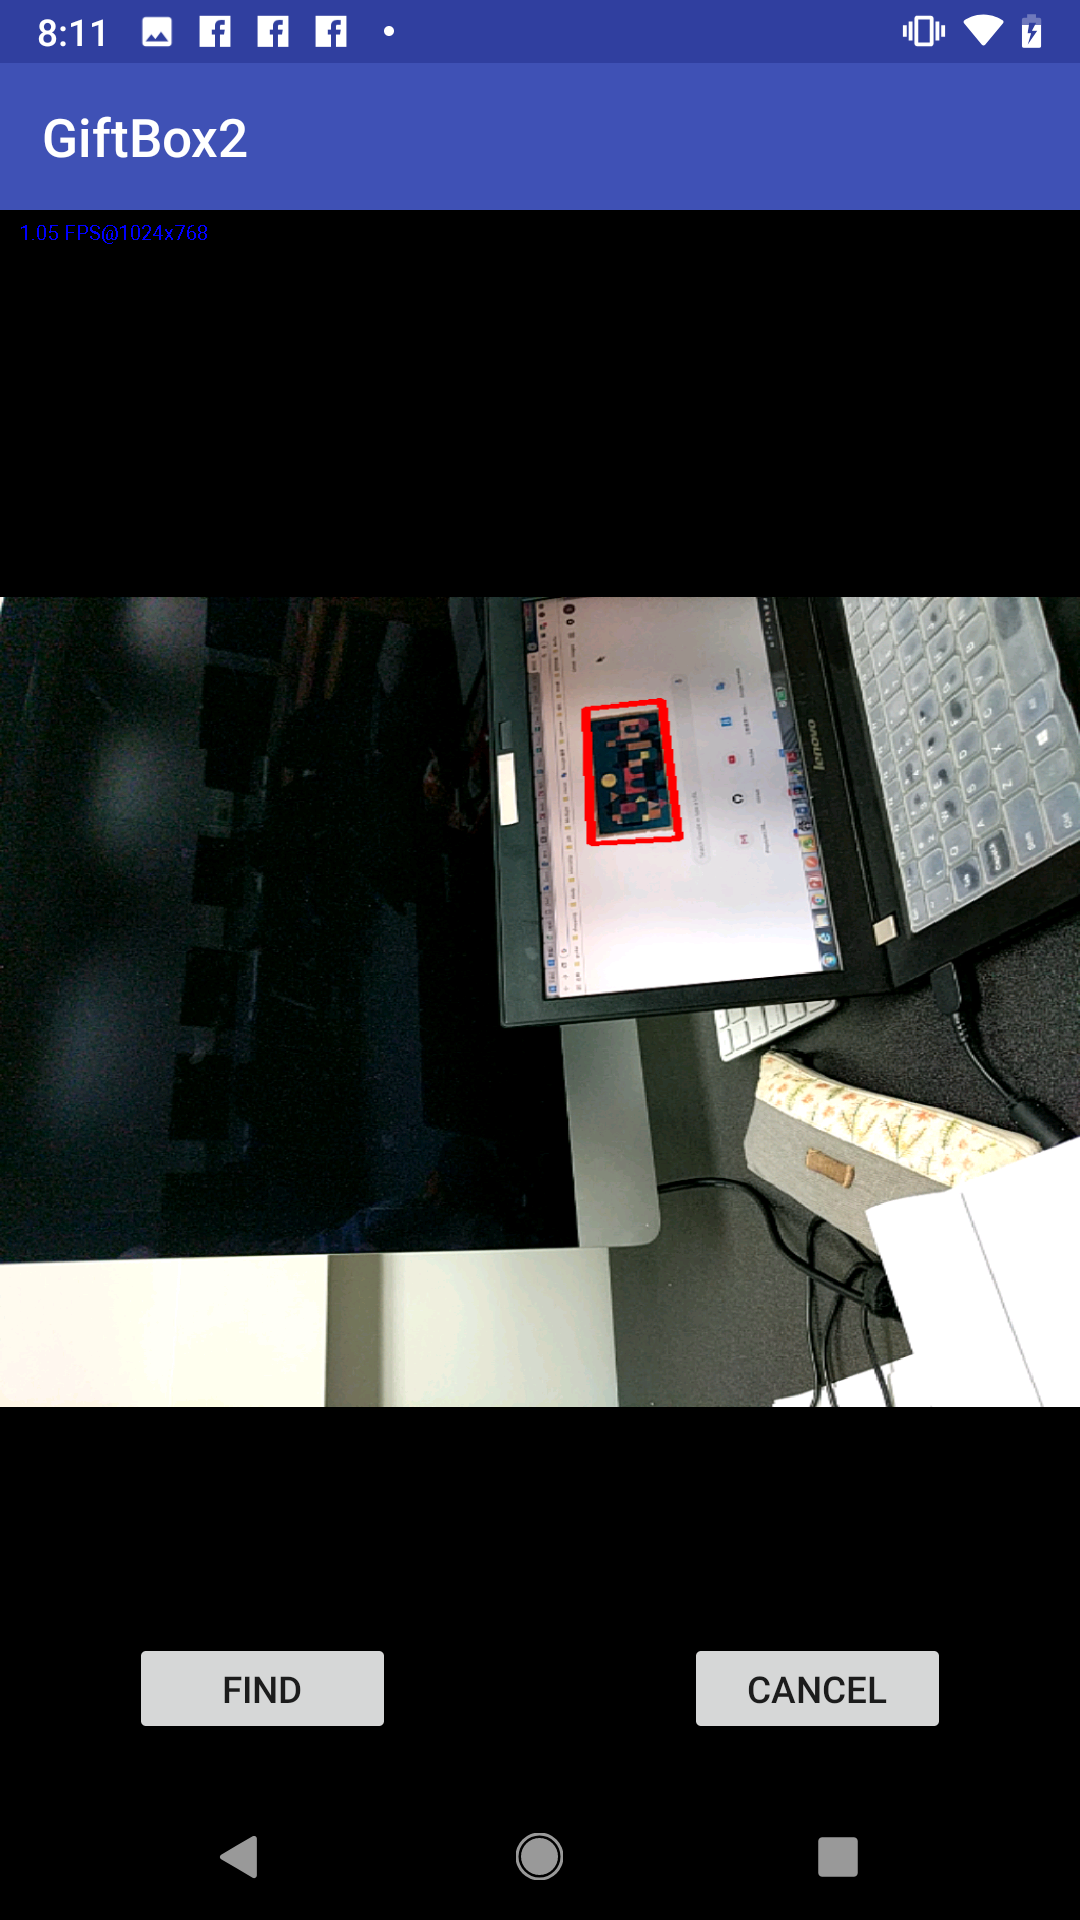
\includegraphics[width=.95\textwidth]{section05/assets/resultExample4.png}
\subcaption{\label{DetectedRegionCorrect2}}
\end{minipage}%
\begin{minipage}[H]{0.3\textwidth}
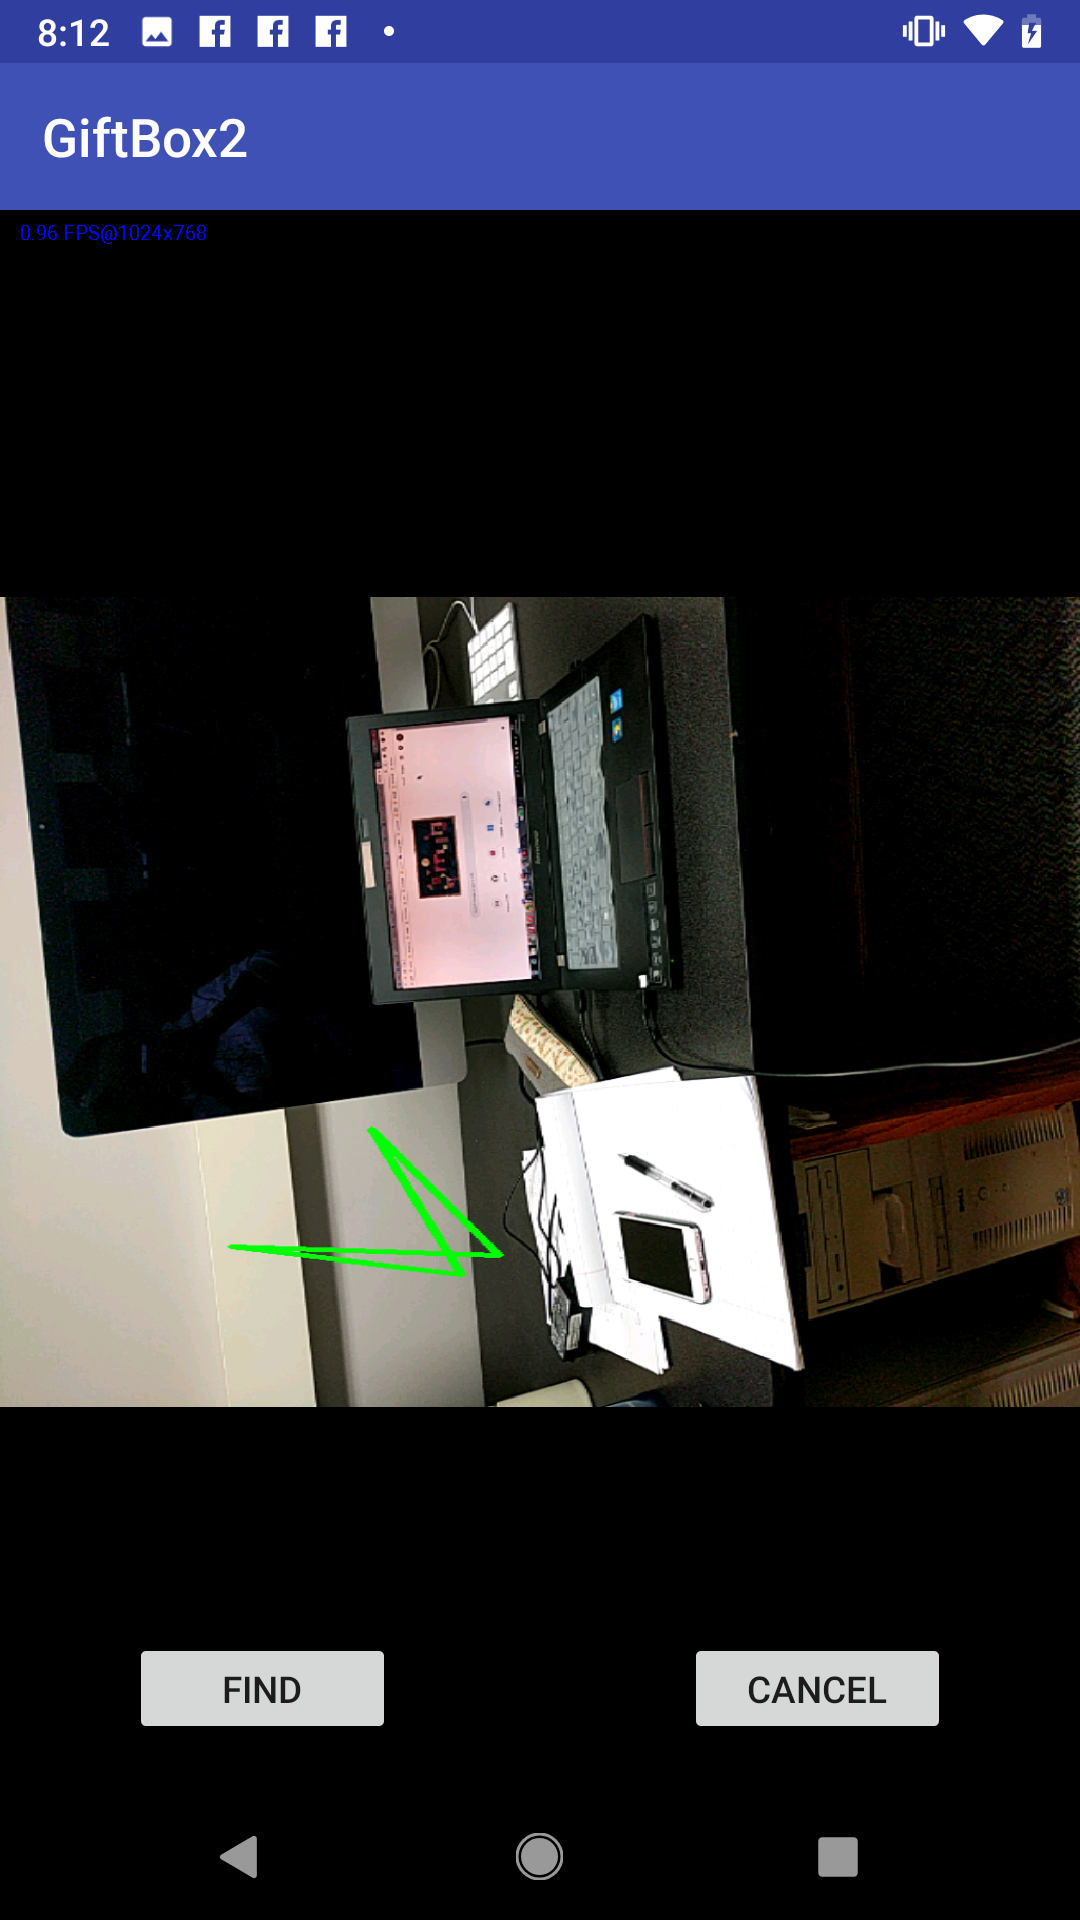
\includegraphics[width=.95\textwidth]{section05/assets/resultExample1.png}
\subcaption{\label{DetectedRegionWrong}}
\end{minipage}%
\caption[An Example for finding a gift]{\label{AnExampleForFindingAGift}An Example for Finding a Gift}
\end{figure}

\par The Figure \ref{AnExampleForFindingAGift} shows an example for finding a gift. Figure \ref{RegionSelected} shows a gift that is being sent and after we send it, the recipient then attempts to find it from different angles. Figure \ref{DetectedRegionCorrect1} shows that the region is correctly recognized if the recipient scans the image from the same location as the sender with the phone rotated from portrait to landscape by the recipient. Figure \ref{DetectedRegionCorrect2} shows that the recipient is able to find the region from a significantly different distance, angle, and orientation. In Figure \ref{DetectedRegionWrong}, we can see that the algorithm gets a wrong result because we are too far away from the selected region. 
\par The web interface was mainly used to retrieve data and show it on the user interface. So we just test it by manual observation. 
